\section{Traction Controller}\label{s:TC}
Sections \ref{s:DTKF} and \ref{s:MME} discuss the DTKF filtering algorithm to estimate slip and terrain-track interaction forces and a way to use these estimates to recrusively estimate terrain conditions for the maximum net traction effort available $F_{net}$ and the peak slip value to produce it $i_{pk}$. This section discusses the controller used to regulate the tractor to the estimated peak slip value $\hat{i}_{pk}$ once the tractor has encountered a softer, low traction terrain. 

A block diagram of the simplified longidtudinal tractor dynamics is shown in Fig. \ref{fig:Open_Loop_Dynamics_TC}. Here, the throttle $\Pi$ and gear ratio selection $g_{GR}$ are the inputs and the tractor speed $v_T$ and driver speed $\dot\varphi$ are the outputs. The engine is considered a time-varying gain depending on the engine operating speed and the transmission is a piecewise constant gain value that is the product of $g_{GR}$ and $g_{FD}$. The approximate continuous range for the engine gain is $K_E \in [1750,2400]$ and the product of $g_{GR}g_{FD}$ takes on discrete values dependent on which gear number 1-16 is being used. The traction controller here will take the form of a PIDF controller. The limited range of continuous engine gains can be handled by a single PIDF controller with fixed gains. However, the range of the the 16 different transmission gains $g_{GR}g_{FD}$ is too large for one controller to handle. Therefore, the controller is gain scheduled based on the the gear ratio $g_{GR}$ selected.
\begin{figure}[b]
    \centering
    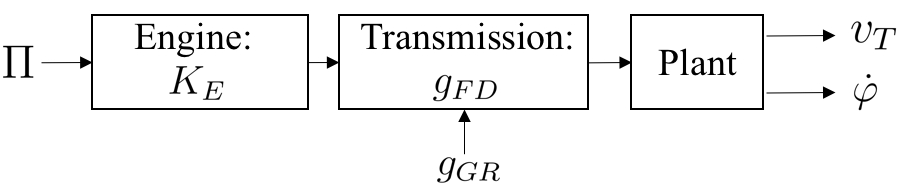
\includegraphics[width = 3.5 in,keepaspectratio]{Open_Loop_Dynamics_TC}
    \caption{Block diagram of the simplified open-loop longitudinal tractor dynamics.}
    \label{fig:Open_Loop_Dynamics_TC}
\end{figure}

The block diagram of the closed-loop system for regulating slip is shown in Fig. \ref{fig:Closed_Loop_Dynamics_TC}. The slip reference $\hat{i}_{pk}$ is the output from MME Bayes' estimator in section \ref{s:MME}. In this control loop, slip is indirectly controlled by regulating the driver speed at the track. To calculate driver speed reference $\dot\varphi_{ref}$ the smoothed velocity estimate $\tilde{v}_T$ is used. 
\begin{equation}
    \dot\varphi_{ref} = \frac{\tilde{v}_T}{r(1-\hat{i}_{pk})}
\end{equation}
The lower limit at each time step is $\dot{\varphi}_{ref}g_{GR}g_{FD} \geq \frac{1300\hspace{1mm} rot}{min}\frac{2\pi\hspace{1mm}rad}{1\hspace{1mm}rot}\frac{1\hspace{1mm}min}{60\hspace{1mm}sec}$ so that the traction controller can not stall out the engine. 
The driver speed error $\dot{\varphi}_e$ is the input to the PIDF controller and is given by
\begin{equation}
    \dot\varphi_e = \dot\varphi_{ref} - \hat{\dot\varphi}
\end{equation}
The output of the PIDF controller $\Pi_{PID}$ is combined with a feed-forward throttle term $\Pi_{FF}$ and is the input to the engine.
\begin{equation}
    \Pi = \Pi_{PID} + \Pi_{FF}
\end{equation}
This feed-forward term is the throttle input being used before the traction controller is turned on and provides a stable transition between the leader-follower and traction control modes. 
\begin{figure}[b]
    \centering
    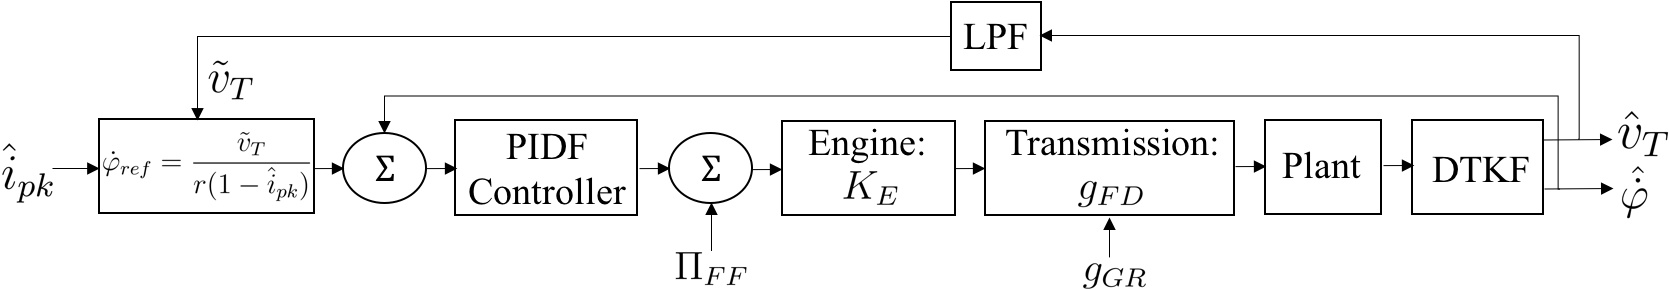
\includegraphics[width = 6 in,keepaspectratio]{Closed_Loop_Dynamics_TC}
    \caption{Block diagram of the closed-loopd dynamics for traction control.}
    \label{fig:Closed_Loop_Dynamics_TC}
\end{figure}

The structure of the PIDF controller is given by
\begin{equation}
    \frac{\Pi_{PID}(s)}{\dot{\varphi}_e(s)} = K_{p,t} + \frac{K_{i,t}}{s} + \frac{K_{d,t}s}{t_fs+1}
\end{equation}
where the derivative term is low pass filtered for stability. The gains selected for the controller are $K_{p,t}=0.28$, $K_{i,t}=0.17$, $K_{d,t}=0.03$, and the filter time constant is $t_f=0.3s$. These gains are divided by the gear ratio $g_{GR}$ in each gear number to have a PIDF controller gain schedule for each gear. This way, the controller will use smaller gain values in gear numbers that have higher gear ratios and larger gain values in higher gear numbers with lower gear ratios. The aim here is that controller performance should be similar across different gear selections. After discretization of the controller, the final result is 16 different sets of controller coefficients for $a_0$, $a_1$, and $a_2$ and $b_0$, $b_1$, and $b_2$
\begin{equation}
    \Pi_{PID}[k] = -\frac{a_1}{a_0}\Pi_{PID}[k-1] -\frac{a_2}{a_0}\Pi_{PID}[k-2]  + \frac{b_0}{a_0}\dot{\varphi}_e[k] + \frac{b_1}{a_0}\dot{\varphi}_e[k-1] + \frac{b_2}{a_0}\dot{\varphi}_e[k-2]
\end{equation}

Gear selections in the traction control mode are based on a desired, bounded engine operating speed $\Omega_E \in [1350,1950]$. If the engine operating speed drifts below the lower bound, the transmission shifts down in gear number and if the engine speed goes above the upper bound it shifts up in gear number. The upper bandwidth of this controller is 0.5 Hz with detection of needed gear changes at 20 Hz. This way, the controller is not limited to only making gear changes at momentary instances every 2 seconds. This is required for operation if there are changes in the tractor's ground speed so that the controller can track updated $\dot{\varphi}_{ref}$ values. 